\documentclass[10pt]{article}
\usepackage[backend=bibtex,style=numeric]{biblatex}
%\usepackage{simplestyle}
\usepackage{enumitem}
\usepackage{graphicx}
\usepackage{caption}
\usepackage{subcaption}
\usepackage{fullpage}

\addbibresource{refs}

\title{Extracting Application and Menu Events from UI Tutorial Videos}
\author{Daniel Seita \& Andrew Head}

\begin{document}

\maketitle

\section{Introduction}

This work seeks to use video processing and object recognition techniques as a technique to
mine the usability of an application.  Given the proliferation of video tutorials on using
different software, this provides new opportunities to assess what complex actions are frequently
performed by a variety of users.  We describe a technique for recognizing menus, detecting that an
item has been clicked in a menu, comparing this menu item to all other instances of that same item
by template matching, and then composing temporally close menu navigations into configuration tasks.
By working with a corpus of around 100 tutorials related to setting up the Eclipse environment for
programming tasks, we describe the configuration tasks that are performed the most often.  We
discuss how we can improve this workflow to improve the speed and accuracy of detection in the
future.

Our contributions include a small but effective dataset for evaluating the effectiveness of
detectors of UI menu-opening actions.

Recent research has focused on how to improve the use of video tutorials to help users learn
software ~\cite{matejka_ambient_2011}~\cite{pongnumkul_pause-and-play_2011}.  One strength of video
tutorials may be that users can directly observe expert use, which can serve as a strong learning
aid~\cite{shneiderman_direct_1983}.  Grossman \& Fitzmaurice showed benefits of short contextual
video clips.  Short, 10-25 second contextually available videos were effective to help users
accomplish task and retain what they learned than traditional text-based
tutorials~\cite{grossman_toolclips_2010}.

However, video tutorials have drawbacks: Navigation issues could lead to misunderstanding of
content~\cite{harrison_comparison_1995}.  Users may not be able to keep up with the pace of the
content~\cite{palmiter_evaluation_1991}.  Researchers working with longer, 2-3 minute task-oriented
tutorials found that users performed better with text tutorials than videos because users could not
work at the same pace as the video~\cite{grabler_generating_2009}.  In general, research on
instructional videos point shows a need to segmented videos to emphasize the steps of the task.

\textbf{Andrew: Make this have less of a strong focus on the value of video tutorials, and instead
talk about mining usability from online data sources, such as with CUTS}


\section{Related Work}

By examining pixels, many have succeeded at reverse engineering user interfaces
and interactions with user interfaces with purely visual information, independent
of any knowledge of underlying application implementation. Work 
by Zettleymoyer et al.~\cite{zettlemoyer_ibots_1999}~\cite{zettlemoyer_visual_1999}
examine widget identification in IBOTS and VisMap.  Also see~\cite{potter_triggers_1992}~\cite{amant_image_2005}~\cite{lieberman_visual_2001}. 
Visual identification of widgets and UIs may also have also been used in Olsen 
et al.'s ScreenCrayons work that links annotations to arbitrary screen 
elements~\cite{olsen_jr_implementing_1999},
and in Tan et al.'s work to interactively subdivide windows with a 
copy-paste metaphor~\cite{tan_wincuts_2004}.
\textbf{Andrew: Check on this.}

More recently, Sikuli~\cite{yeh_sikuli_2009} uses computer vision to 
identify GUI elements from screen captures, using template matching for small
UI elements and voting based on invariant local features for large elements.
In application, Sikuli allows users to search for documentation related to
screenshots taken of UI elements, and to script GUI tasks using visual
cues of the UI.  For searching based on screenshots, 3 types of features are 
extracted: text from the source document, visual words computed from visual 
words from MSER-detected salient elliptical patches, and 3-grams over widget-embedded 
text extracted through OCR.  For searching on the screen for saved 
screenshot images, small patterns are found via template matching and large 
patterns through invariant feature voting.

Pause-and-Play extends the template matching approach of Sikuli to detect 
tool-selection UI events in compressed, low-resolution video tutorials.  
The system takes a tool palette template and tool icons as input, 
producing metadata file of tool changes with timecodes.  With template 
matching at multiple resolutions, detection is invariant to recording 
resolution and some camera effects.  Their system cannot be run in in 
real-time~\cite{pongnumkul_pause-and-play_2011}.

A number of different technologies attempt to learn templates for arbitrary UI 
elements~\cite{chang_associating_2011}~\cite{dixon_prefab_2010}~\cite{hurst_automatically_2010}~\cite{matejka_ambient_2011}.
Learning may require access to mouse APIs~\cite{hurst_automatically_2010}
and accessibility APIs~\cite{chang_associating_2011}.

Prefab identifies GUI elements with GUI specific visual features~\cite{dixon_prefab_2010}, which 
enables overlay of advanced interactions on existing interfaces~\cite{dixon_content_2011}~\cite{dixon_general-purpose_2012}.
\textbf{Andrew: Check up on this initial description.  I'm also not sure
if Prefab actually belongs in this conceptual group.}
To delve into the technical implementations of the Prefab pixel-based 
matching algorithm, we report from~\cite{dixon_general-purpose_2012}.
Prefab identifies interface elements using a library of prototypes.  
This uses two strategies: exact matches of prototype pixels against an image,
and modelining the prototype background and differencing pixel in an image 
to identify foreground interface elements.  
Prefab generalizes from example images to models which contain parts like 
exact pixel features, or regions or areas of variable size or repeating 
patterns.  It organizes the entire interface into a hierarchy.

Waken contributes to this space by discovering 
cursor shapes, clicking actions, icons, tooltips and menus, all by examining 
the difference between frames of UI video.  They do this by making assumptions 
about how the image of icons change during hover and press actions.  Detection 
of the cursor and icons in later frames is performed by template matching~\cite{banovic_waken_2012}.
We rely on techniques similar to those in Waken to establish when menus
have been activated and menu items selected.


\section{Video Classification}

This will be Daniel's section. I'm probably not going to include any subsections to save time.

Figure~\ref{fig:alex_net} shows our accuracy results for the two AlexNet networks we trained.

Figure~\ref{fig:per_class} shows our per-class accuracy results for the ``no noise'' AlexNet
network.

\begin{figure}
\centering
  \begin{minipage}{.45\textwidth}
  \centering
  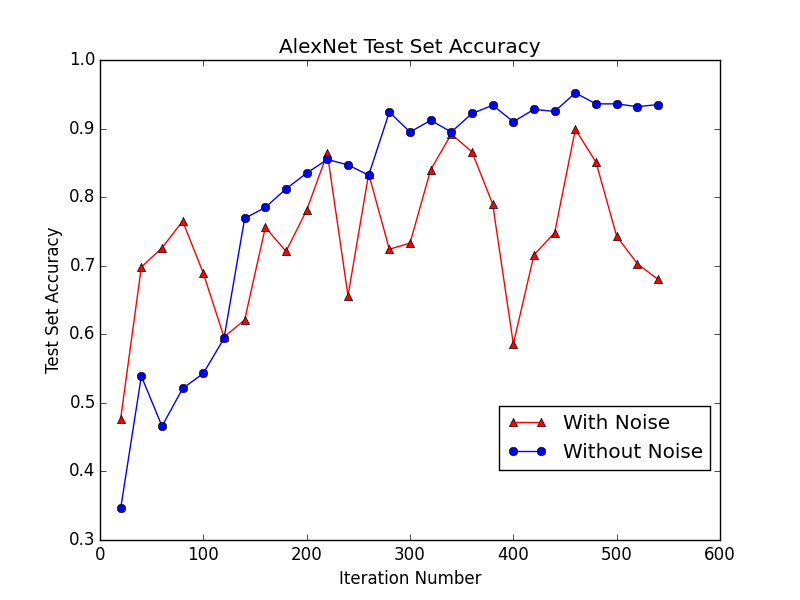
\includegraphics[width=1\linewidth]{AlexNet_Accuracy}
  \caption{AlexNet accuracy results of two networks trained on two image datasets.}
  \label{fig:alex_net}
  \end{minipage}\hfill
  \begin{minipage}{.45\textwidth}
  \centering
  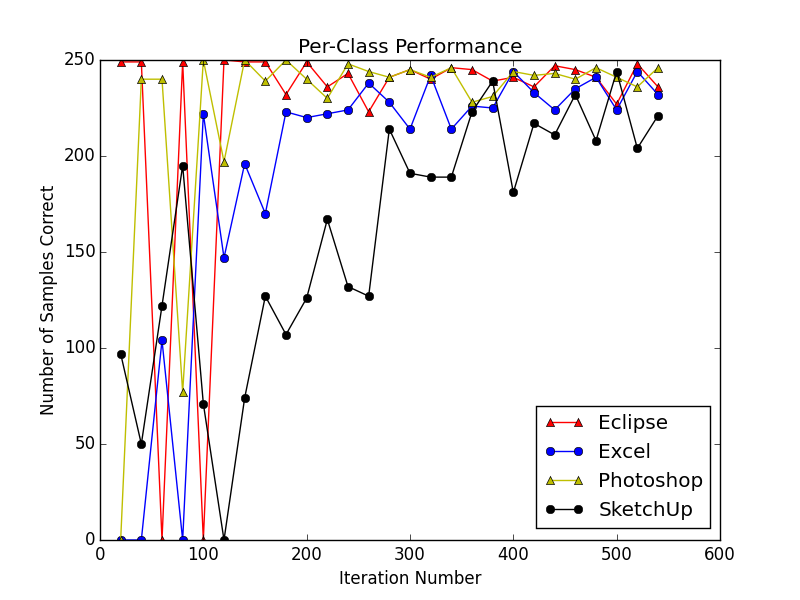
\includegraphics[width=1\linewidth]{PerClassPerformance}
  \caption{AlexNet per-class accuracy results for the network trained on ``no noise'' data.}
  \label{fig:per_class}
  \end{minipage}
\end{figure}

Figures~\ref{fig:filters_all} and~\ref{fig:filters_nonoise} show visualizations of the 96 filters in
the first layer of AlexNet, each of which has dimension $55\times 55$.

\begin{figure}
\centering
  \begin{minipage}{.4\textwidth}
  \centering
  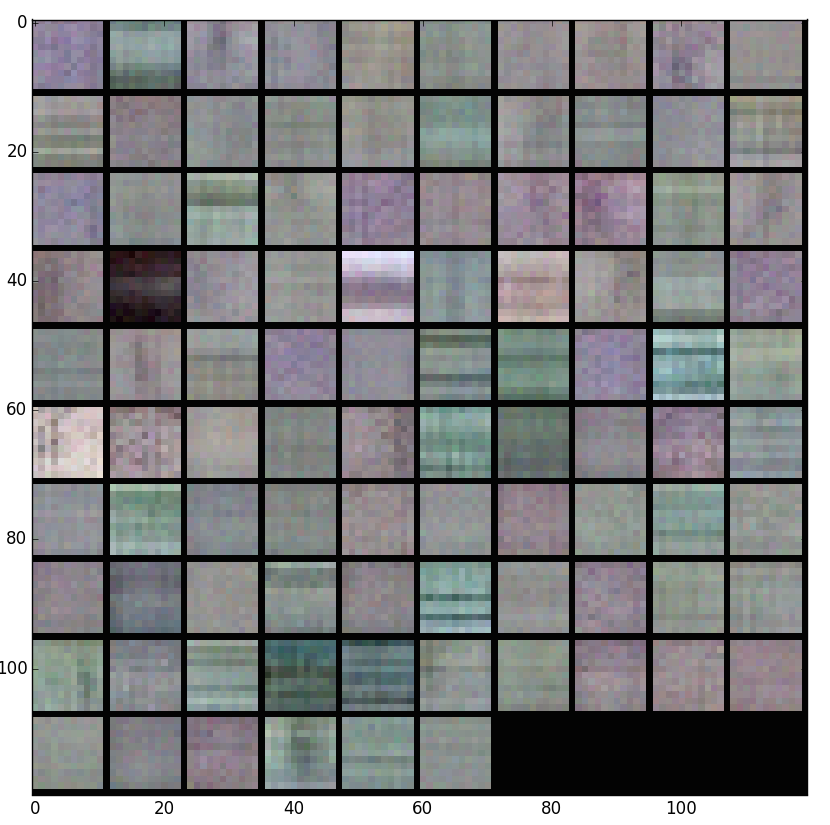
\includegraphics[width=1\linewidth]{Filters_All}
  \caption{Visualization of filters from the network trained on all our image data.}
  \label{fig:filters_all}
  \end{minipage}\hfill
  \begin{minipage}{.4\textwidth}
  \centering
  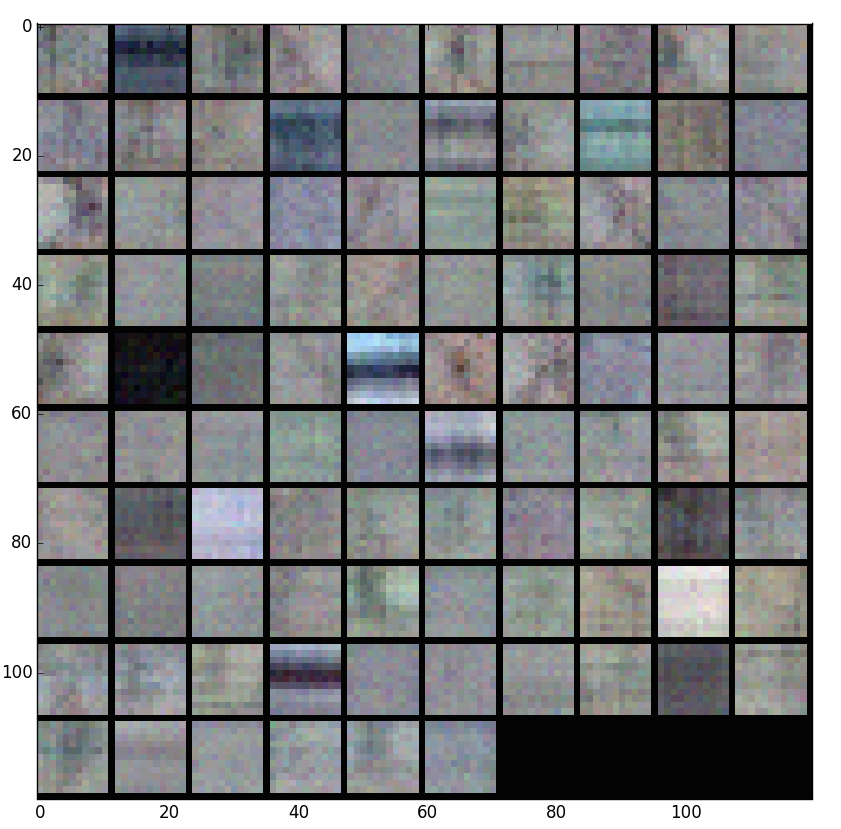
\includegraphics[width=1\linewidth]{Filters_NoNoise}
  \caption{Visualization of filters from the network trained on ``no noise'' image data.}
  \label{fig:filters_nonoise}
  \end{minipage}
\end{figure}


\section{Locating Menus in a Frame Sequence}

This will be Andrew's section.

\subsection{Data}

Answer these questions:
\begin{enumerate}[noitemsep]
\item What is our dataset?
\item How did we construct/acquire it?
\item What's its size?
\item (optional) How will we improve it in the future?
\end{enumerate}


\subsection{Implementation}
Here's a figure of our (edit: Andrew's) pipeline.  \textbf{Andrew: Add figure of pipeline.}

\subsection{Menu Location Results}

Here we (edit: Andrew) want to touch upon:
\begin{enumerate}[noitemsep]
\item How reliably can we classify UI events?
\item How long does it take for us to process one minute of video?  What are
the practical implications of this?
\item Some images that show recognition results for a few representative
screenshots of user interfaces.
\end{enumerate}


\section{Discussion and Conclusion}

TODO (combining the two because we don't have a lot of space!)

We freakin' rock.

\printbibliography

\end{document}
